\chapter{Persamaan Garis Lurus}

\section*{Pengantar}

Persamaan garis lurus merupakan salah satu konsep paling mendasar dalam matematika rekayasa dan menjadi titik awal yang tepat untuk mempelajari buku ini. Garis lurus adalah representasi geometris dari fungsi linear, dan kemampuan untuk menentukan persamaan garis, menghitung jarak, serta memahami hubungan antar garis sangat dibutuhkan dalam analisis teknik. Bab ini membahas berbagai bentuk persamaan garis lurus, operasi geometris yang melibatkan garis, serta perluasan ke kurva parabola sebagai pengantar menuju konsep fungsi yang lebih umum pada Bab~2.

\section{Bentuk Umum Persamaan Garis}

Bentuk umum persamaan garis lurus adalah
\begin{equation}
    ax+by+c = 0,
\end{equation}
dengan $a$, $b$, $c$ adalah bilangan real. Persamaan di atas dapat diubah menjadi:
$$ by = -ax -c. $$ 
Jika semua suku dibagi dengan $b$ maka
$$ y = -\frac{a}{b}x - \frac{c}{b}, $$
di mana $-a/b$ merupakan \textbf{gradien} garis $= \tan \theta = m$, dengan $\theta$ adalah sudut positif antara garis dan sumbu $x$.

\begin{center}
\begin{tabular}{ l c r }
\raisebox{-.5\height}{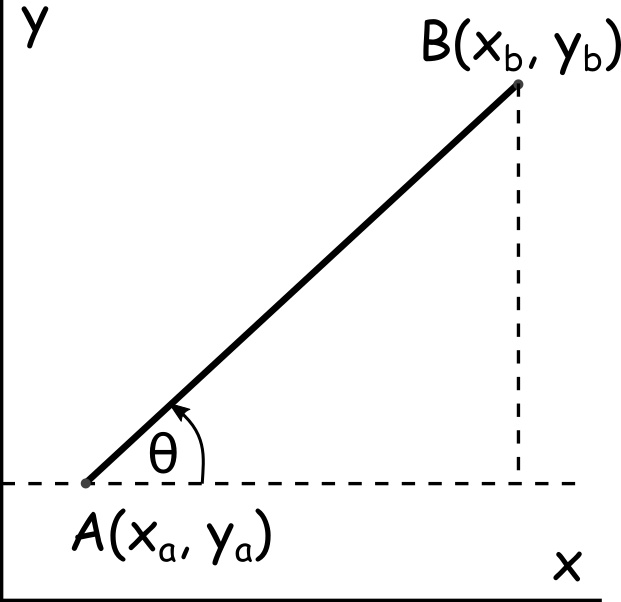
\includegraphics[width=2in]{pict/m1}} & & $m = \dfrac{y_B-y_A}{x_B-x_A}=\dfrac{y_A-y_B}{x_A-x_B}$
\end{tabular}
\end{center}

\section{Persamaan Garis Lewat $(x_0, y_0)$ dengan Gradien $m$}

\begin{equation}
    y-y_0=m(x-x_0). \label{eq:garis-titik-gradien}
\end{equation}

\begin{exmp}
Tentukan persamaan garis yang melalui titik $(2, 3)$ dengan gradien $m = -1$!

\textbf{Penyelesaian:}\\
Dengan Persamaan~\ref{eq:garis-titik-gradien}:
\[
y - 3 = -1(x - 2) \;\Longrightarrow\; y = -x + 5.
\]
\end{exmp}

\section{Persamaan Garis Lewat Dua Titik $(x_A, y_A)$ dan $(x_B, y_B)$}

Substitusikan $m = (y_B - y_A)/(x_B - x_A)$ ke dalam Persamaan~\ref{eq:garis-titik-gradien} untuk memperoleh:
\begin{equation}
\frac{y-y_A}{y_B - y_A} = \frac{x - x_A}{x_B - x_A}.
\end{equation}

\begin{exmp}
Tentukan persamaan garis yang melalui $A(1, 2)$ dan $B(4, 8)$!

\textbf{Penyelesaian:}\\
\[
m = \frac{8-2}{4-1} = 2, \quad y - 2 = 2(x - 1) \;\Longrightarrow\; y = 2x.
\]
\end{exmp}

\section{Sudut Antara Dua Garis}

Jika diketahui dua garis:
\begin{align*}
g&: \quad ax + by + c = 0 \;\rightarrow\; m_1= -\frac{a}{b}, \\
l&: \quad px + qy + r = 0 \;\rightarrow\; m_2= -\frac{p}{q},
\end{align*}
maka sudut $\theta$ antara kedua garis diberikan oleh:
\begin{equation}
\tan \theta = \frac{m_2 - m_1}{1+m_1 m_2}.
\end{equation}

\textbf{Bukti:} Misalkan $\alpha$ dan $\beta$ adalah sudut yang dibentuk oleh garis $g$ dan $l$ terhadap sumbu $x$ positif, sehingga $m_1 = \tan\alpha$ dan $m_2 = \tan\beta$. Sudut antara kedua garis adalah $\theta = \beta - \alpha$. Dengan rumus selisih tangen:
\[
\tan\theta = \tan(\beta - \alpha) = \frac{\tan\beta - \tan\alpha}{1 + \tan\alpha\,\tan\beta} = \frac{m_2 - m_1}{1 + m_1 m_2}. \qed
\]

Dua garis dikatakan \textbf{sejajar} jika $m_1 = m_2$, dan \textbf{tegak lurus} jika $m_1 \cdot m_2 = -1$.

\begin{exmp}
Tentukan sudut antara garis $y = 2x + 1$ dan $y = -x + 3$!

\textbf{Penyelesaian:}\\
Dengan $m_1 = 2$ dan $m_2 = -1$:
\[
\tan\theta = \frac{-1 - 2}{1 + (2)(-1)} = \frac{-3}{-1} = 3.
\]
Sehingga $\theta = \arctan 3 \approx 71{,}57^\circ$.
\end{exmp}

\section{Jarak Titik $(x_0, y_0)$ ke Garis $ax+by+c=0$}

Jarak $d$ dari titik $(x_0, y_0)$ ke garis $ax+by+c=0$ dirumuskan:
\begin{equation}
    d = \frac{|a\,x_0+b\,y_0+c|}{\sqrt{a^2+b^2}}.
\end{equation}

\begin{exmp}
Hitunglah jarak dari titik $(3, 4)$ ke garis $3x + 4y - 5 = 0$!

\textbf{Penyelesaian:}\\
\[
d = \frac{|3(3) + 4(4) - 5|}{\sqrt{9 + 16}} = \frac{|9 + 16 - 5|}{5} = \frac{20}{5} = 4.
\]
\end{exmp}

\section{Persamaan Garis Bagi Sudut}

Untuk dua garis $g: ax + by + c = 0$ dan $l: px + qy + r = 0$, persamaan garis bagi sudut (tempat kedudukan titik-titik yang berjarak sama dari kedua garis) adalah:
\begin{equation}
    \frac{ax+by+c}{\sqrt{a^2+b^2}} = \pm\frac{px+qy+r}{\sqrt{p^2+q^2}}.
\end{equation}
Tanda positif dan negatif menghasilkan dua garis bagi yang saling tegak lurus.

\section{Persamaan Berkas Garis}

Setiap garis yang melewati titik potong garis $g$ dan $l$ dapat dinyatakan sebagai \textbf{berkas garis}:
\begin{equation}
    g + \lambda\,l = 0,
\end{equation}
dengan $\lambda$ adalah parameter yang ditentukan dari syarat tambahan (misalnya garis harus melalui titik tertentu).

\begin{exmp}
Tentukan persamaan garis yang melalui titik potong garis $x + y - 2 = 0$ dan $2x - y + 1 = 0$ serta melalui titik $(0, 5)$!

\textbf{Penyelesaian:}\\
Berkas garis: $(x + y - 2) + \lambda(2x - y + 1) = 0$. Substitusi $(0, 5)$:
\[
(0 + 5 - 2) + \lambda(0 - 5 + 1) = 0 \;\Longrightarrow\; 3 - 4\lambda = 0 \;\Longrightarrow\; \lambda = \frac{3}{4}.
\]
Persamaan garis: $(x + y - 2) + \frac{3}{4}(2x - y + 1) = 0$, atau disederhanakan: $10x + y - 5 = 0$.
\end{exmp}

\section{Pergeseran Grafik}

\subsection{Pergeseran ke Kanan dan ke Kiri}

Pergeseran grafik fungsi $y = f(x)$ ke \textbf{kanan} sejauh $a$ satuan menghasilkan grafik $y = f(x - a)$. Sebaliknya, pergeseran ke \textbf{kiri} sejauh $a$ satuan menghasilkan $y = f(x + a)$.

\begin{figure}[!h]
\begin{center}
    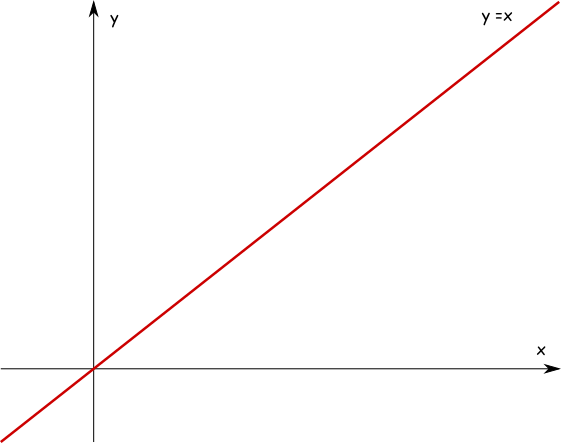
\includegraphics[width=3in]{pict/grafik1}
    \caption{Grafik persamaan garis $y=x$} \label{fig:grafik1}
\end{center}
\end{figure}

Jika setiap titik pada garis $y = x$ digeser sejajar sumbu $x$ ke kanan sejauh 2 satuan, maka:
\[
x \rightarrow (x-2), \quad \text{sehingga}\quad y = x - 2,
\]
seperti ditunjukkan pada Gambar~\ref{fig:grafik1-2}.
\begin{figure}[!h]
\begin{center}
    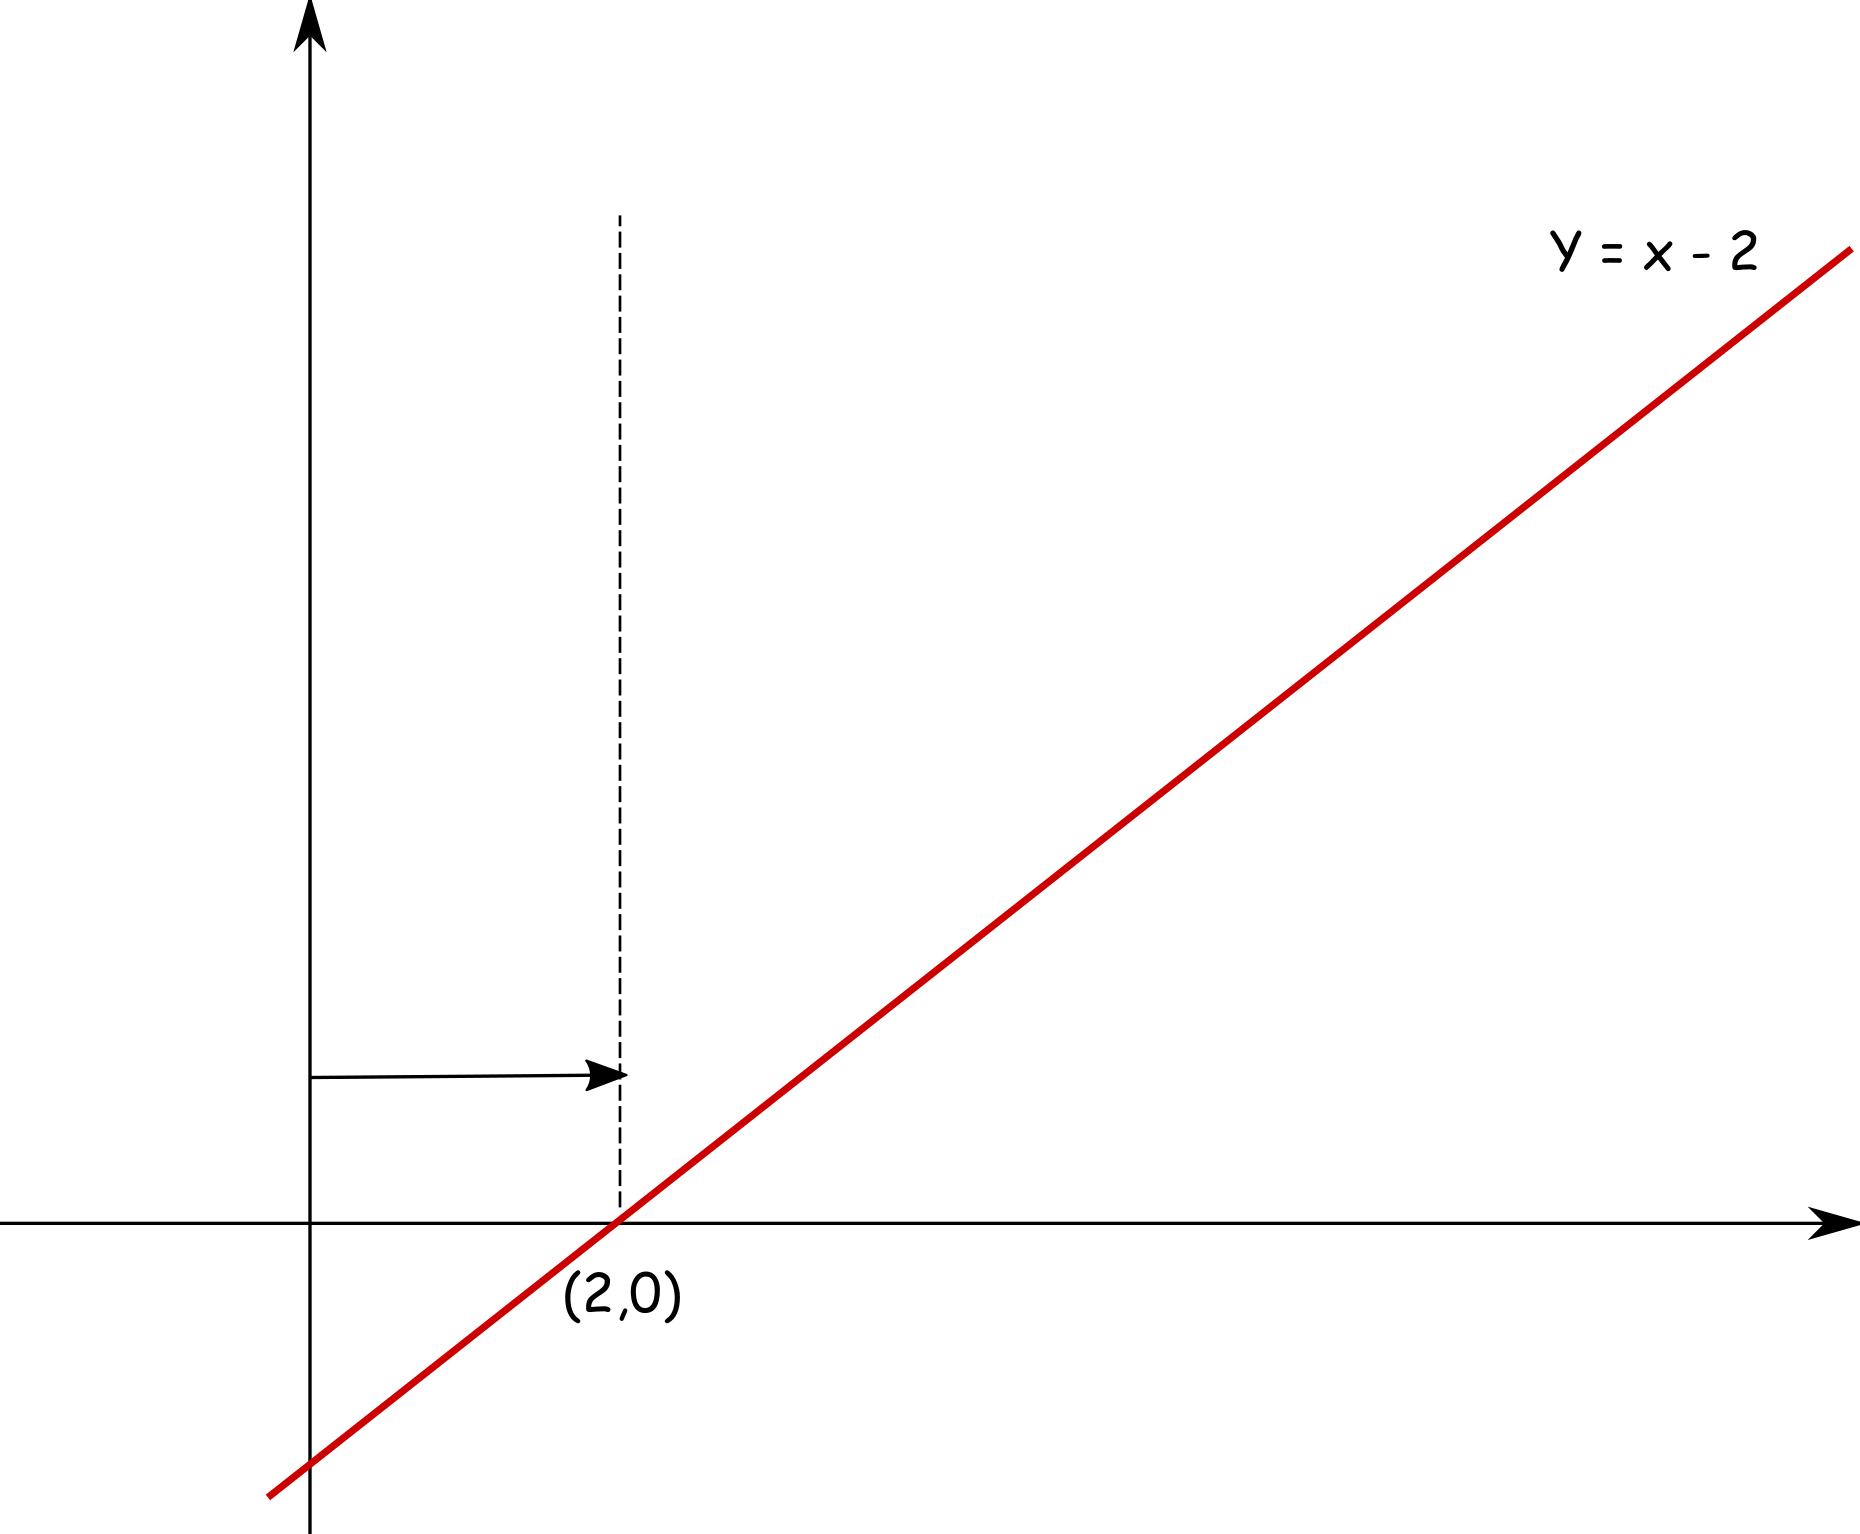
\includegraphics[width=3in]{pict/grafik1-2}
    \caption{Grafik persamaan garis $y=x-2$ (hasil pergeseran ke kanan sejauh 2)} \label{fig:grafik1-2}
\end{center}
\end{figure}

\subsection{Pergeseran ke Atas dan ke Bawah}

Pergeseran grafik $y = f(x)$ ke \textbf{atas} sejauh $b$ satuan menghasilkan $y = f(x) + b$, dan ke \textbf{bawah} sejauh $b$ satuan menghasilkan $y = f(x) - b$.

Sebagai contoh, $y = x$ digeser ke bawah sejauh 2 satuan menjadi $y = x - 2$, atau secara ekuivalen $y + 2 = x$, seperti ditunjukkan pada Gambar~\ref{fig:grafik1-3}.

\begin{figure}[!h]
\begin{center}
    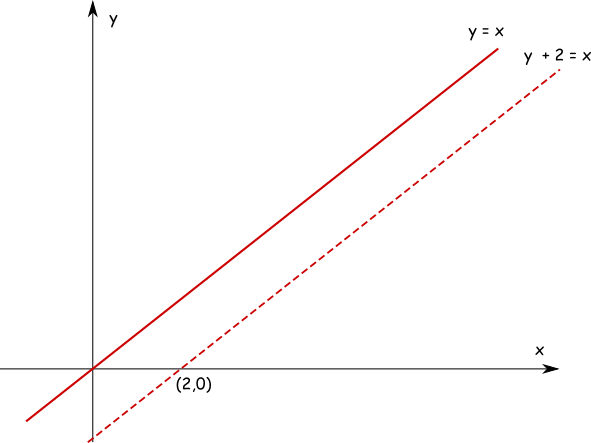
\includegraphics[width=3in]{pict/grafik1-3}
    \caption{Grafik persamaan garis $y+2=x$ (hasil pergeseran ke bawah sejauh 2)} \label{fig:grafik1-3}
\end{center}
\end{figure}

Prinsip pergeseran ini berlaku untuk semua fungsi $y = f(x)$, tidak terbatas pada garis lurus. Konsep ini akan sangat berguna ketika kita mempelajari fungsi-fungsi yang lebih umum pada Bab~2.

\section{Grafik Parabola}

Parabola merupakan perluasan dari konsep garis lurus menuju kurva kuadrat. Pemahaman parabola menjadi penting karena merupakan contoh pertama dari \textit{fungsi nonlinear} yang akan dibahas lebih lanjut pada Bab~2 (Fungsi).

\subsection{Parabola dengan Sumbu Simetri Sejajar Sumbu $x$}

\textbf{Definisi:} Parabola adalah tempat kedudukan titik-titik yang berjarak sama terhadap satu titik (\textbf{fokus}) dan satu garis (\textbf{direktriks}).

\begin{center}
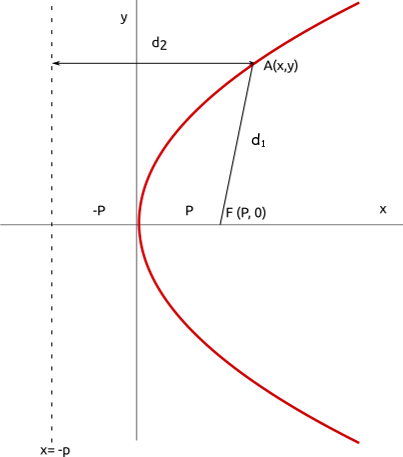
\includegraphics[width=3in]{pict/parabola3}
\end{center}

Agar titik $A(x,y)$ berada pada parabola (sesuai definisi), maka $d_1 = d_2$:
\begin{align*}
d_1 &= \sqrt{(x-p)^2 + y^2}, \\
d_2 &= x + p.
\end{align*}
Dari $d_1 = d_2$:
\[
(x+p)^2 = (x-p)^2 + y^2 \;\Longrightarrow\; x^2 + 2xp + p^2 = x^2 - 2xp + p^2 + y^2,
\]
sehingga diperoleh:
\begin{equation}
 y^2 = 4px.
\end{equation}
Ini adalah persamaan parabola dengan puncak $(0,0)$, fokus $(p,0)$, dan direktriks $x = -p$.

Jika puncak digeser ke $(a,b)$ maka persamaannya menjadi:
\begin{equation}
    (y-b)^2 = 4p(x-a),
\end{equation}
dengan fokus $F(p+a,\, b)$, direktriks $x = -p + a$, dan sumbu simetri $y = b$.

Jika $p > 0$, parabola terbuka ke kanan; jika $p < 0$, parabola terbuka ke kiri.

\begin{exmp}
Tentukan puncak, fokus, dan persamaan direktriks dari $y^2 - 4y - 8x - 4 = 0$!

\textbf{Penyelesaian:}\\
Lengkapkan kuadrat untuk $y$:
\[
(y^2 - 4y + 4) = 8x + 4 + 4 \;\Longrightarrow\; (y-2)^2 = 8(x+1).
\]
Sehingga puncak $= (-1, 2)$, $4p = 8 \Rightarrow p = 2$, fokus $= (1, 2)$, dan direktriks $x = -3$.
\end{exmp}

\subsection{Parabola dengan Sumbu Simetri Sejajar Sumbu $y$}

\begin{center}
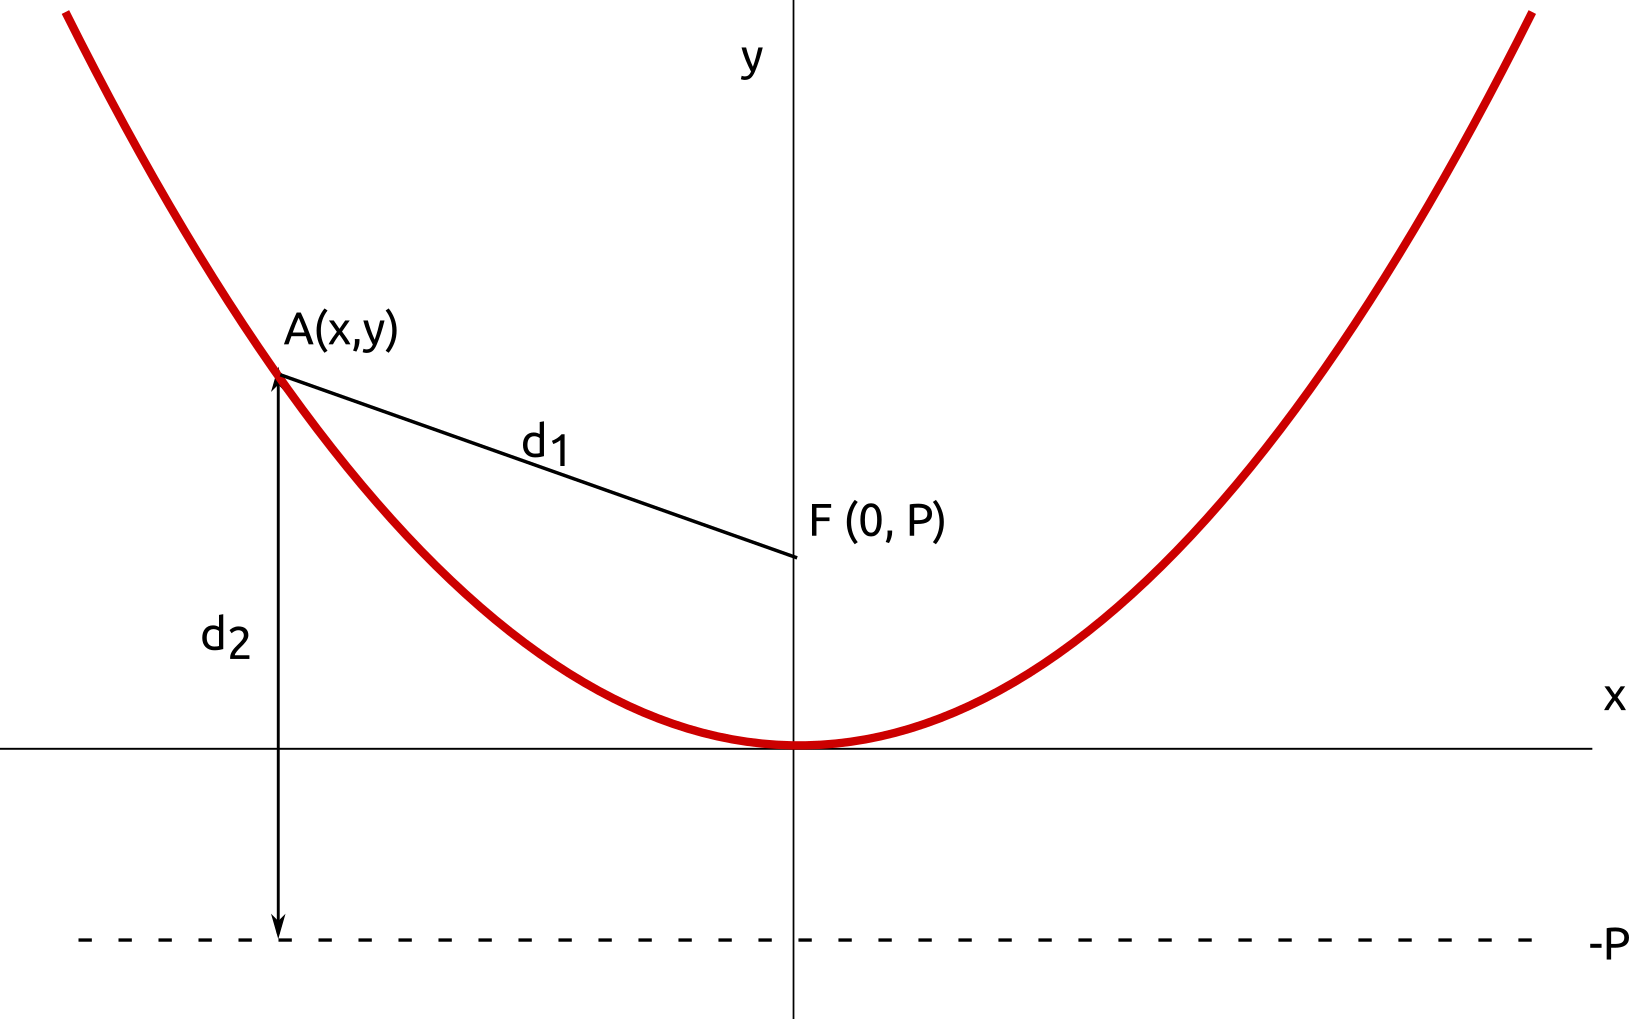
\includegraphics[width=3in]{pict/parabola4}
\end{center}

Dengan cara yang analog, diperoleh:
\begin{equation}
x^2 = 4py \quad\Longrightarrow\quad y = \frac{1}{4p}\,x^2.
\end{equation}
Ini adalah persamaan parabola dengan sumbu simetri sejajar sumbu $y$, fokus $(0,p)$, dan direktriks $y = -p$.

Jika puncak digeser ke $(a,b)$:
\begin{equation}
(y-b) = \frac{1}{4p}(x-a)^2,
\end{equation}
dengan fokus $F(a,\, b+p)$, direktriks $y = -p+b$, dan sumbu simetri $x = a$.

\subsection{Bentuk Lain Persamaan Parabola}

Bentuk umum $y = ax^2 + bx + c$ (dengan $a \ne 0$) dapat ditulis ulang dengan melengkapkan kuadrat:
\begin{equation}
y = a\left(x+\frac{b}{2a}\right)^2-\frac{D}{4a},
\end{equation}
dengan $D = b^2 - 4ac$ adalah diskriminan. Koordinat puncak parabola adalah $\left(-\dfrac{b}{2a},\, -\dfrac{D}{4a}\right)$.

\begin{exmp}
Tentukan puncak dan sketsa grafik dari $y = x^2 - 6x + 14$!

\textbf{Penyelesaian:}\\
Dengan $a = 1$, $b = -6$, $c = 14$: $D = 36 - 56 = -20$.
\[
\text{Puncak} = \left(\frac{6}{2},\, \frac{20}{4}\right) = (3,\, 5).
\]
Karena $a > 0$, parabola terbuka ke atas dengan titik minimum di $(3, 5)$.
\end{exmp}

\section*{Rangkuman}

Persamaan garis lurus dapat dinyatakan dalam berbagai bentuk: bentuk umum $ax + by + c = 0$, bentuk titik-gradien $y - y_0 = m(x - x_0)$, dan bentuk dua titik. Konsep gradien ($m = \tan\theta$) merupakan kunci untuk memahami kemiringan garis. Sudut antara dua garis, jarak titik ke garis, garis bagi sudut, dan berkas garis merupakan operasi geometris penting. Prinsip pergeseran grafik, baik horizontal maupun vertikal, berlaku umum untuk semua fungsi. Parabola sebagai kurva kuadrat merupakan jembatan menuju konsep fungsi nonlinear yang lebih umum.

\section*{Latihan Soal}

\begin{enumerate}
  \item Tentukan persamaan garis yang melalui titik $(3, -1)$ dan tegak lurus terhadap garis $2x - 3y + 5 = 0$!
  \item Hitunglah jarak dari titik $(1, 1)$ ke garis $3x + 4y - 12 = 0$!
  \item Garis $y = x + 5$ terbentuk jika $y = x$ digeser ke arah mana dan sejauh berapa?
  \item Gambarkan grafik: (a) $y = x^2$, (b) $y = (x-1)^2$, (c) $y = (x-1)^2 - 4$. Jelaskan pergeseran yang terjadi!
  \item Tentukan fokus, direktriks, dan sumbu simetri dari $y = 4x^2 - 4x - 3$!
  \item Tentukan persamaan kurva berikut:
  \begin{center}
    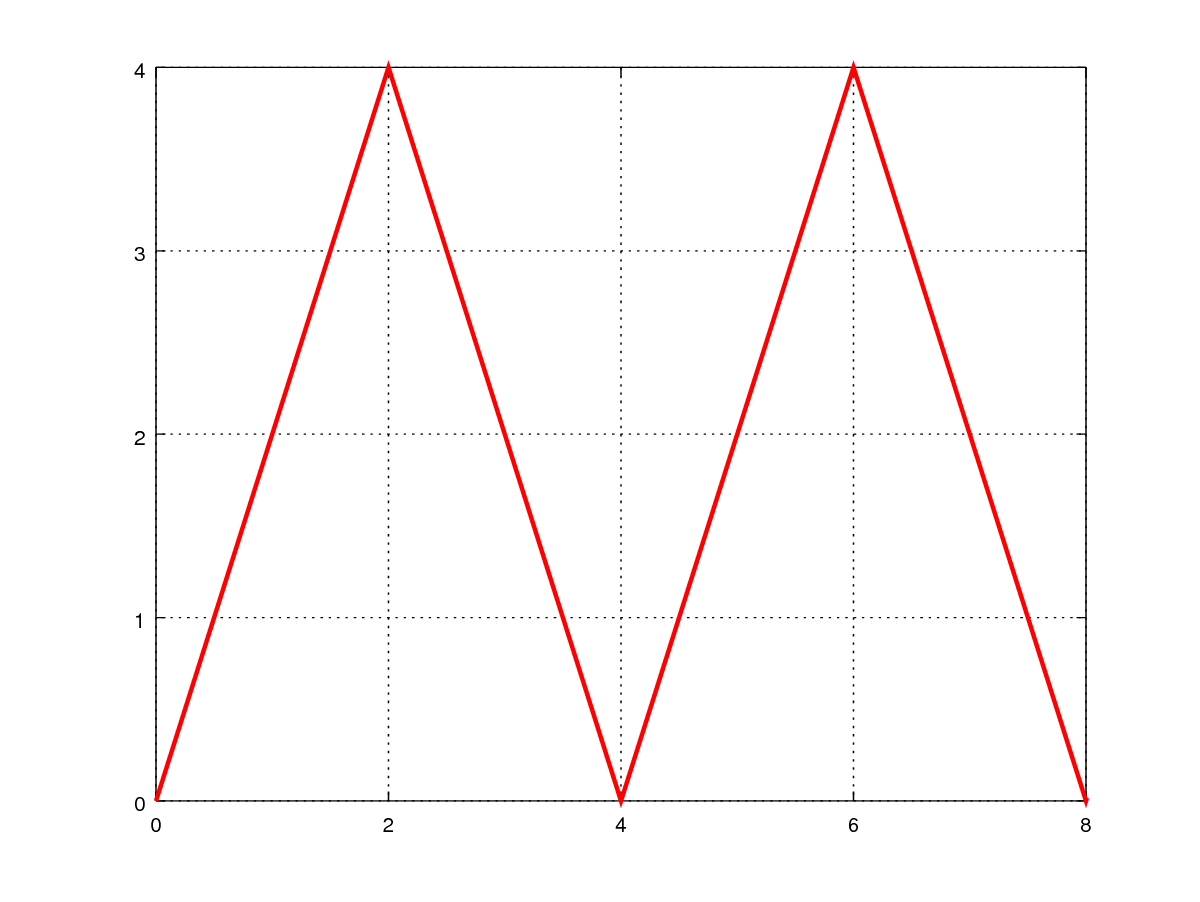
\includegraphics[width=3.5in]{pict/triangle.png}
  \end{center}
  \item Jika $A(2,1)$, $B(10,6)$, dan $C(4,12)$, tentukan luas segitiga $ABC$!
\end{enumerate}
